\documentclass[unicode,11pt,a4paper,oneside,numbers=endperiod,openany]{scrartcl}

\renewcommand{\thesubsection}{\arabic{subsection}}

\usepackage{ifthen}
\usepackage[utf8]{inputenc}
\usepackage{graphics}
\usepackage{graphicx}
\usepackage{hyperref}

\pagestyle{plain}
\voffset -5mm
\oddsidemargin  0mm
\evensidemargin -11mm
\marginparwidth 2cm
\marginparsep 0pt
\topmargin 0mm
\headheight 0pt
\headsep 0pt
\topskip 0pt        
\textheight 255mm
\textwidth 165mm

\newcommand{\duedate} {}
\newcommand{\setduedate}[1]{%
\renewcommand\duedate {\textbf{Due date:}~ #1}}
\newcommand\isassignment {false}
\newcommand{\setassignment}{\renewcommand\isassignment {true}}
\newcommand{\ifassignment}[1]{\ifthenelse{\boolean{\isassignment}}{#1}{}}
\newcommand{\ifnotassignment}[1]{\ifthenelse{\boolean{\isassignment}}{}{#1}}

\newcommand{\assignmentpolicy}{
\begin{table}[h]
\begin{center}
\scalebox{0.8} {%
\begin{tabular}{|p{0.02cm}p{16cm}|}
\hline
&\\
\multicolumn{2}{|c|}{\Large\textbf{Numerical Computing 2023 ---  Submission Instructions}}\\
\multicolumn{2}{|c|}{\large\textbf{(Please, notice that following instructions are mandatory: }}\\
\multicolumn{2}{|c|}{\large\textbf{submissions that don't comply with, won't be considered)}}\\
&\\
\textbullet & Assignments must be submitted to \href{https://www.icorsi.ch/course/view.php?id=14666}{iCorsi} (i.e. in electronic format).\\
\textbullet & Provide both executable package and sources (e.g. C/C++ files, MATLAB). 
If you are using libraries, please add them in the file. Sources must be organized in directories called:\\
\multicolumn{2}{|c|}{\textit{Project\_number\_lastname\_firstname}}\\
& and  the  file must be called:\\
\multicolumn{2}{|c|}{\textit{project\_number\_lastname\_firstname.zip}}\\
\multicolumn{2}{|c|}{\textit{project\_number\_lastname\_firstname.pdf}}\\
\textbullet &  The TAs will grade your project by reviewing your project write-up, and looking at the implementation you attempted, and benchmarking your code's performance.\\

\textbullet & You are allowed to discuss all questions with anyone you like; however: (i) your submission must list anyone you discussed problems with and (ii) you must write up your submission independently.\\
\hline
\end{tabular}
}
\end{center}
\end{table}
}
\newcommand{\punkte}[1]{\hspace{1ex}\emph{\mdseries\hfill(#1~\ifcase#1{Points}\or{Points}\else{Points}\fi)}}


\newcommand\serieheader[6]{
\thispagestyle{empty}%
\begin{flushleft}

\includegraphics[width=0.45\textwidth]{CI_logo}
\end{flushleft}
  \noindent%
  {\large\ignorespaces{\textbf{#1}}\hspace{\fill}\ignorespaces{ \textbf{#2}}}\\ \\%
  {\large\ignorespaces #3 \hspace{\fill}\ignorespaces #4}\\
  \noindent%
  \bigskip
  \hrule\par\bigskip\noindent%
  \bigskip {\ignorespaces {\Large{\textbf{#5}}}
  \hspace{\fill}\ignorespaces \large \ifthenelse{\boolean{\isassignment}}{\duedate}{#6}}
  \hrule\par\bigskip\noindent%  \linebreak
 }

\makeatletter
\def\enumerateMod{\ifnum \@enumdepth >3 \@toodeep\else
      \advance\@enumdepth \@ne
      \edef\@enumctr{enum\romannumeral\the\@enumdepth}\list
      {\csname label\@enumctr\endcsname}{\usecounter
        {\@enumctr}%%%? the following differs from "enumerate"
	\topsep0pt%
	\partopsep0pt%
	\itemsep0pt%
	\def\makelabel##1{\hss\llap{##1}}}\fi}
\let\endenumerateMod =\endlist
\makeatother




\usepackage{textcomp}







\usepackage{float}



\begin{document}


\setassignment
\setduedate{Friday, December 29, 2023, 11:59 PM}

\serieheader{Numerical Computing}{2023}{Student: Harkeerat Singh Sawhney}{Discussed with: FULL NAME}{Solution for Project 5}{}
\newline

\assignmentpolicy

\newpage

\section{Graphical Solution of Linear Programming Problems [20 points]}
\subsection{Problem 1}
\subsubsection{Solve the System of Inequalities}
We are asked to solve the system of inequalities, which is already given in the question itself.

\begin{equation}
	\begin{aligned}
		min \quad  & z = 4x + y      \\
		s.t. \quad & x + 2y \leq 40  \\
		           & x + y \geq 30   \\
		           & 2x + 3y \geq 72 \\
		           & x, y \geq 0
	\end{aligned}
	\label{eq:1.1.1}
\end{equation}

Hence as it can be seen from the Equation \ref{eq:1.1.1}, we have to find the minimum value of $z$ such that the constraints are satisfied. This can be solved graphically by plotting the constraints and finding the minimum value of $z$. Before that lets rewrite the constraints in the form of $y = mx + c$ which can be seen at Equation \ref{eq:1.1.2}.

\begin{equation}
	\begin{aligned}
		min \quad  & z = 4x + y             \\
		s.t. \quad & y = -\frac{1}{2}x + 20 \\
		           & y = -x + 30            \\
		           & y = -\frac{2}{3}x + 24 \\
		           & x, y \geq 0
	\end{aligned}
	\label{eq:1.1.2}
\end{equation}

\subsubsection{Plot the feasible region identified by the constraints.}

\begin{figure}[H]
	\centering
	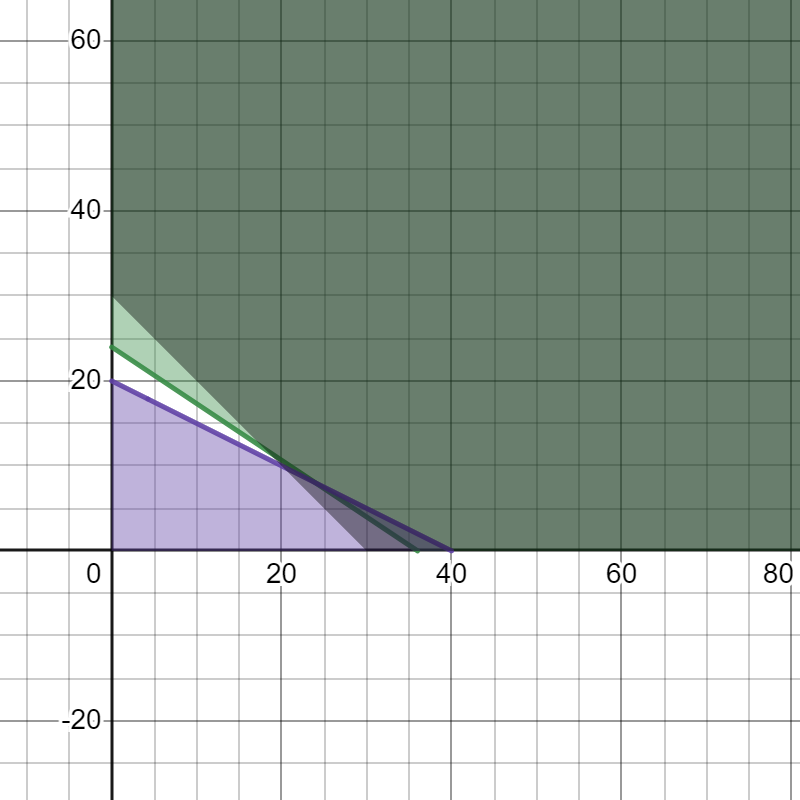
\includegraphics[width=0.5\linewidth]{figures/problem_1.1.1.png}
	\caption{Plot of all the constraints for Problem 1}
	\label{fig:problem_1.1}
\end{figure}
Now we can plot the constraints on a graph as shown in Figure \ref{fig:problem_1.1}. Figure \ref{fig:problem_1.1} is showing the plot of all the constraints. All of these constraints can be seen by their respective colors. However what we are interested is in the region where all the constraints maximum, as that region would include all minimum value of $z$.

\begin{figure}[H]
	\centering
	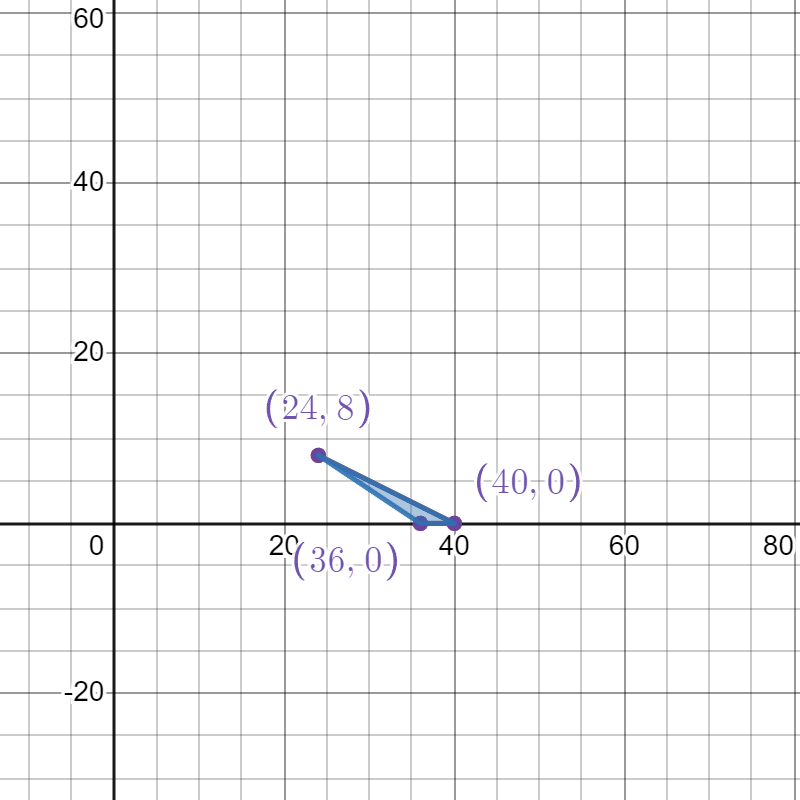
\includegraphics[width=0.5\linewidth]{figures/problem_1.1.2.png}
	\caption{Shading the region where all the constraints maximum for Problem 1}
	\label{fig:problem_1.2}
\end{figure}

As it can be seen from the Figure \ref{fig:problem_1.2}, the region where all the constraints maximum is the region where the minimum value of $z$ would be. Here what is important for us is the points of intersection of the constrains with each other and the points of intersection of the constraints with the axes. These points are as well shown in the Figure \ref{fig:problem_1.2}. These points are as follows:

\begin{itemize}
	\item $(24, 8)$
	\item $(40, 0)$
	\item $(36, 0)$
\end{itemize}

\subsubsection{ Find the optimal solution and the value of the objective function in that point.}
Now from the previous part we have the points of intersection of the constraints with each other and the points of intersection of the constraints with the axes. What we need to do now is to find the minium value of $z$ at these points. Hence we have to evaluate the objective function at each vertices and pick the minimum value of $z$. The vertices are as follows:

\begin{equation}
	\begin{aligned}
		At \quad (24, 8) \quad z = 4(24) + 8 = 104 \\
		At \quad (40, 0) \quad z = 4(40) + 0 = 160 \\
		At \quad (36, 0) \quad z = 4(36) + 0 = 144
	\end{aligned}
	\label{eq:1.1.3}
\end{equation}

From the Equation \ref{eq:1.1.3} we can see that the minimum value of $z$ is at $(24, 8)$ which is $104$.

\subsection{Problem 2}
\subsubsection{Solve the System of Inequalities}
This is a bit more tricker than the previous problem, as unlike previous problem we do now have the mathematical form of the constraints. We have a real life problem from which we have to convert to the mathematical form. The problem is as follows:

\begin{quote}
	\textit{A tailor plans to sell two types of trousers, with production costs of $25 $ CHF and $40$ CHF, respectively. The former type can be sold for $85$ CHF, while the latter for $110$ CHF. The tailor estimates a total monthly demand of $265$ trousers. Find the number of units of each type of trousers that should be produced in order to maximize the net profit of the tailor, if we assume that the he cannot spend more than $7000$ CHF in raw materials.?}
\end{quote}

Hence from the above problem we can see that we have to find the maximum value of $z$ which is the net profit of the tailer. The variables are as follows:


\begin{itemize}
	\item $x$ = Number of trousers of type 1
	\item $y$ = Number of trousers of type 2
	\item $z$ = Net profit of the tailor
\end{itemize}

We have obtained the Objective Function (Maximize Profit $z$) by knowing that the profit from selling the first type of trousers is $85 - 25 = 60$ CHF and the profit from selling the second type of trousers is $110 - 40 = 70$ CHF. Hence we can write the Objective Function as follows:

\begin{equation}
	\begin{aligned}
		Maximize \quad & z = 60x + 70y \\
	\end{aligned}
	\label{eq:1.1.4}
\end{equation}

We know that the total demand of trousers is $265$ and the total amount of money that can be spent on raw materials is $7000$ CHF. Hence we can write the first constraint as follows:

\begin{equation}
	\begin{aligned}
		x + y \leq 265 \\
	\end{aligned}
	\label{eq:1.1.5}
\end{equation}

We also know that the cost of producing the first type of trousers is $25$ CHF and the cost of producing the second type of trousers is $40$ CHF. Hence we can write the second constraint as follows:

\begin{equation}
	\begin{aligned}
		25x + 40y \leq 7000 \\
	\end{aligned}
	\label{eq:1.1.6}
\end{equation}

Hence finally by combining the Equation \ref{eq:1.1.4}, \ref{eq:1.1.5} and \ref{eq:1.1.6} we can write the constraints as follows in the mathematical form at Equation \ref{eq:1.1.7}.

\begin{equation}
	\begin{aligned}
		min \quad  & z = 60x + 25y       \\
		s.t. \quad & x + y \leq 265      \\
		           & 25x + 40y \leq 7000 \\
		           & x, y \geq 0
	\end{aligned}
	\label{eq:1.1.7}
\end{equation}

Now we must rewrite the constraints in the form of $y = mx + c$ which can be seen at Equation \ref{eq:1.1.8}.

\begin{equation}
	\begin{aligned}
		min \quad  & z = 60x + 25y           \\
		s.t. \quad & y = -x + 265            \\
		           & y = -\frac{5}{8}x + 175 \\
		           & x, y \geq 0
	\end{aligned}
	\label{eq:1.1.8}
\end{equation}

\subsubsection{Plot the feasible region identified by the constraints.}

\begin{figure}[H]
	\centering
	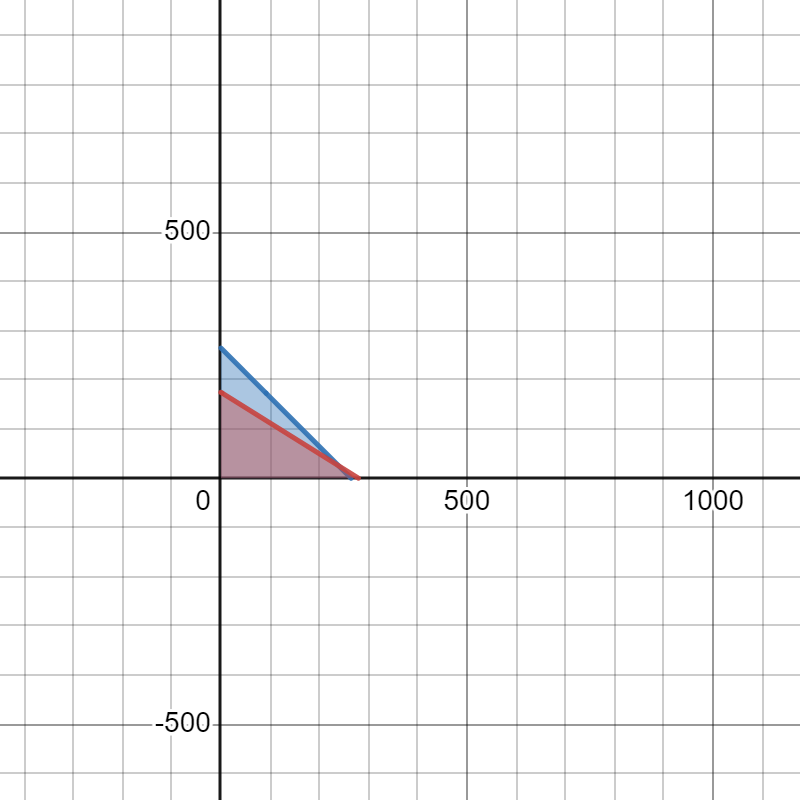
\includegraphics[width=0.5\linewidth]{figures/problem_1.2.1.png}
	\caption{Plot of all the constraints for Problem 2}
	\label{fig:problem_2.1}
\end{figure}

Again very similar to the previous problem, we have to plot the constraints on a graph as shown in Figure \ref{fig:problem_2.1}. Figure \ref{fig:problem_2.1} is showing the plot of all the constraints and all of these constraints can be seen by their respective colors. However what we are interested is in the region where all the constraints maximum, as that region would include all maximize value of $z$.

\begin{figure}[H]
	\centering
	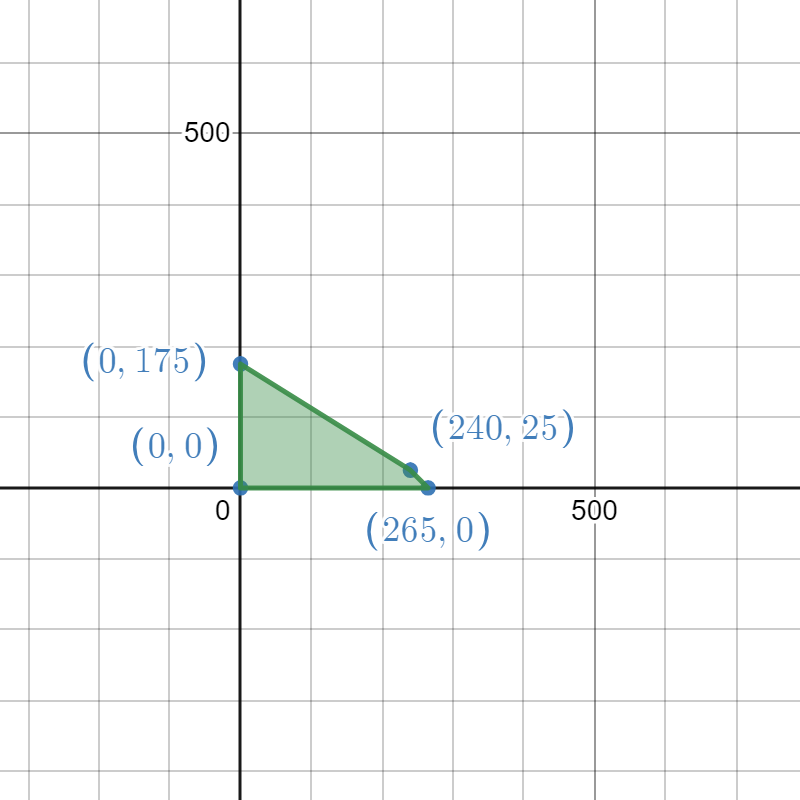
\includegraphics[width=0.5\linewidth]{figures/problem_1.2.2.png}
	\caption{Shading the region where all the constraints maximum for Problem 2}
	\label{fig:problem_2.2}
\end{figure}

As it can be seen from the Figure \ref{fig:problem_2.2}, the region where all the constraints maximum is the region where the maximum value of $z$ would be. Here what is important for us is the points of intersection of the constrains with each other and the points of intersection of the constraints with the axes. These points are as well shown in the Figure \ref{fig:problem_2.2}. These points are as follows:

\begin{itemize}
	\item $(0, 175)$
	\item $(240, 25)$
	\item $(265, 0)$
	\item $(0, 0)$
\end{itemize}

\subsubsection{ Find the optimal solution and the value of the objective function in that point.}

Now from the previous part we have the points of intersection of the constraints with each other and the points of intersection of the constraints with the axes. What we need to do now is to find the minium value of $z$ at these points. Hence we have to evaluate the objective function at each vertices and pick the minimum value of $z$. The vertices are as follows:

\begin{equation}
	\begin{aligned}
		At \quad (0, 175) \quad z = 60(0) + 25(175) = 4375    \\
		At \quad (240, 25) \quad z = 60(240) + 25(25) = 15025 \\
		At \quad (265, 0) \quad z = 60(265) + 25(0) = 15900   \\
		At \quad (0, 0) \quad z = 60(0) + 25(0) = 0
	\end{aligned}
	\label{eq:1.1.9}
\end{equation}

From the Equation \ref{eq:1.1.9} we can see that the maximum value of $z$ is at $(265, 0)$ which is $15900$.





\end{document}
